\documentclass[a4paper,11pt]{article}

\usepackage{mlsubmit}

\begin{document}

\initmlsubmision{2}                                       % assignment number
                {Nikhil Mittal}                               % your name
                {17111056}                                    % your roll number

\begin{mlsolution}

1. Answer : NO. It is useful only when the Name exists in the data, but if the name is not present then we can't classify based on name. So the first attribute (name) is not useful in learning.
If we build a decision tree using the attribute name then the branching factor will be such high that it will shatter any dataset and overfit.
\\

2. Answer : No.\\
    
    Consider rows $4$ and $6$,\
    we see, other than name, all the attribute are same, but label is no and yes, respectively.
    So without using the label 'name' we can not classify the given data. And name is not useful in learning.
    
    However, if we consider only these 15 rows with name as an attribute, we can always get a perfect classification.

3. Decision Tree obtained after ID3 decision tree learning algorithm is shown in Figure 1. Steps for producing this are :
\\\\Attributes are : Size of research group, Like the research area, Average workload, No. of meetings  per week. Suppose S is this full data given. Then, \\\\Entropy(S) = 0.9182\\
Gain(S, Size of research group) = 0.0679\\
Gain(S, Like the research area) = 0.03170\\
Gain(S, Average workload) = 0.06131\\
Gain(S, No. of meetings  per week) = 0.2516\\\\So Root node is No. of meetings per week as it has the highest Gain.\\\\Since "No. of meetings per week" has three possible values, the root node has three branches (2-3, 0-1, $>$3). All rows with 2-3 meetings per week give result "NO", and similarly on taking branch "$>$3" we get "NO" as answer. \\\\We only decide on the remaining three attributes: Size of research group, Like the research area, Average workload. S is now the remaining set under branch "0-1" (No. of meetings per week).\\
Entropy(S) = 1.0\\
Gain(S, Size of research group) = 0.11452\\
Gain(S, Like the research area) = 0.0348\\
Gain(S, Average workload) = 0.439\\\\Selecting Average workload as the decision node. Splitting into branches upon its possible values. "Average" workload branch leads to always "Yes" as answer.\\Still need to decide for "Heavy" and "Light" average workload branch.\\\\For "Heavy" (Average workload) branch :\\Entropy(S) = 0.7219\\
Gain(S, Size of research group) = 0.1709\\
Gain(S, Like the research area) = 0.0729\\\\Selecting Size of research group as the decision node, highest gain.
Its branches are Medium and Large. Large always yields "NO" and Medium gives "YES" for 1 data point and "NO" for 2 data points, hence choosing "NO" by majority.\\\\For "Light" (Average workload) branch :\\
Entropy(S) = 1.0\\
Gain(S, Size of research group) = 0\\
Gain(S, Like the research area) = 1.0\\\\Selecting Like the research area as the decision node, highest gain. We have Yes and No as branches and it's values are "NO" and "YES" one for each data point respectively. So arbitrarily breaking tie by choosing "YES".\\\\Since we have to stop splitting nodes that are at depth 2 or more. Hence this "Light" Average workload branch always results in "YES" as answer, hence assigning directly to "YES" without any further split. Similarly the "Heavy" Average workload branch always results in "NO" as answer irrespective of the "Size of Research group" being Medium or Large, hence directly assigning the leaf node answer "NO" without any further split.\\\\These steps give us the decision tree as shown in figure 1.

\begin{figure}[th]%
\centering
\includegraphics[width=0.5\columnwidth]{tree.png}%

\caption{Decision Tree}%
\label{fig:Dtree}%
\end{figure}
\end{mlsolution}

\begin{mlsolution}

1.
Story :

The latent variable is the list of items which user purchased.

\[
\mathbb{P} (b^{i} | x^{i}, \theta) = \sum_{k=1}^{2^{L}} \mathbb{P}\left ( b^{i}, z^{i} = S^k | x^{i}, \theta \right ) 
\]

\[
= \sum_{k=1}^{2^{L}} \mathbb{P} \left ( b^{i} | z^{i}=S^k, x^{i}, \theta \right )*\mathbb{P} \left ( z^{i}=S^k | x^{i}, \theta \right )
\]
\\
s.t. $z^{i}.C \leq b^{i}$

This constraint can be solved using lagrangian method as seen as class. 

$\mathbb{P} \left ( b^{i} | z^{i}=S^k, x^{i}, \theta \right )
$ is the likelihood of the cost for a possible list of items. \\

$\mathbb{P} \left ( z^{i}=S^k | x^{i}, \theta \right )$ is the probability of the list $S^k$ for user $x^{i}$.\\

\[
\mathbb{P} \left ( z^{i}| x^{i}, \theta \right ) = \prod_{j=1}^{|z^i|} p^{z^i_j} (1 -
 p )^{1 - z^i_j}
\]

$p = \sigma(t)$ (sigmoid function)\\

2. Write down the complete likelihood expression for the observed data 
\[
\mathbb{P}[b^{i}|x^{i}, W] = \frac{1}{2\pi\sigma^{2}}\exp( - \frac{(b^{i} - \left \langle  W[i], C\right \rangle)^{2}}{\sigma^{2}})
\]

\[
\mathbb{P}[b|X, W] = \prod_{i=1}^{n} \frac{1}{2\pi\sigma^{2}}\exp( - \frac{(b^{i} - \left \langle  W[i], C\right \rangle)^{2}}{\sigma^{2}})
\]

C is the cost vector of items.

3. Hard-assignment alternating optimization algorithm\\

i) Initialize $\theta^{0} = [W^{0,0}, W^{0,1}, ... , W^{0, 2^L-1}]$\\

ii) For i \in $[n]$, \text{update}\; $z^{i,t}$ using $\theta^{t}$
    Let $z^{i,t}$ = \arg \max_{k \in [2^L]} \mathbb{P} [b^{i} | x^{i}, W^{k,t}] 

iii) \[
W^{t+1, k} = \arg \min_{w} \sum_{i:z^{i,t} = k} (b^i - \left \langle W, C \right \rangle)^2 + \sum_{i=1}^{n}\lambda_{i}(z_{i}.C - b)
\]

iv) Set $\theta^{t+1} = [W^{t+1,0}, W^{t+1,1}, ... , W^{t+1, 2^L-1}]$\\

v) Repeat until convergence.
\end{mlsolution}

\begin{mlsolution}

\[
f(w) = \arg \underset{w, {\xi_{i} }}{\min} \left \| w \right \|_{2}^{2} + \sum_{i = 1}^{n} \xi^{2}
\]\[
\\
s.t. y^{i} \left \langle w, x^{i} \right \rangle \geq 1 - \xi_{i}, \text{for} \; \text{all} \; i \in [n]
\]\[\\
\xi_{i} \geq 0\; \text{for} \; \text{all} \; i \in [n]
\]

\textbf{2.3.2}: Answer :\\

Lagrangian for (P1) :

\[
\mathcal{L}(w, \xi, \alpha, \beta) = \arg \underset{w, {\xi_{i} }}{ \text{min} } \; \underset{\alpha\geq 0 ,\; \beta\geq0}{\text{max}} \; \left \| w \right \|_{2}^{2} + \sum_{i = 1}^{n} \xi^{2}
 - \sum_{i=1}^{n} \alpha_{i} \left ( y^{i} \left \langle w, x^{i} \right \rangle - 1 + \xi_{i} \right ) - \sum_{i=1}^{n}\beta_{i} \xi_{i}
\]\\

\textbf{2.3.3}: Answer :\\

Derivation for Dual problem for (P1)\\

We can solve this problem by taking gradients.Since our goal is to remove the dependence on w, the first step is to take a gradient with respect to w, set it equal to zero, and solve for w in terms of the other variables.\\
\[
\frac{\partial  \mathcal{L}}{\partial w} = 2w - \sum_{i=1}^{n} \alpha_{i}y^{i}x^{i} 
\]\\\[
\frac{\partial  \mathcal{L}}{\partial w}  = 0
\]\\\[
w = \frac{1}{2}\sum_{i=1}^{n} \alpha_{i}y^{i}x^{i} 
\]\\

Also to remove the dependence on $\xi$, take a gradient with respect to $\xi$, set it equal to zero, and solve for $\xi$ in terms of the other variables.\\

\[
\frac{\partial  \mathcal{L}}{\partial \xi_{i} } = 2\;\xi_{i} - \alpha_{i} - \beta_{i}
\]\\\[
\frac{\partial  \mathcal{L}}{\partial \xi_{i} } = 0
\]\\\[
\xi_{i} = \frac{\alpha_{i} + \beta_{i}}{2}
\]\\

Substitute w and $\xi$ back in $\mathcal{L}(w, \xi, \alpha, \beta)$ and eliminate them.\\

\[
  \mathcal{L}\left ( \alpha,\; \beta  \right ) = \underset{\alpha\geq 0, \beta \geq 0 }{\text{max}} \left ( \frac{1}{2}\sum_{i=1}^{n} \alpha_{i}y^{i}x^{i}  \right )\left ( \frac{1}{2}\sum_{j=1}^{n} \alpha_{j}y^{j}x^{j} \right ) + \sum_{i=1}^{n} \left ( \frac{\alpha_{i} + \beta_{i}}{2} \right )^{2}  \]\\\[ - \sum_{i=1}^{n} \alpha_{i}\left ( y^{i}\left ( \frac{1}{2}\sum_{j=1}^{n} \alpha_{j}y^{j}x^{j}  \right )x^{i} - 1  +  \frac{\alpha_{i} + \beta_{i}}{2} \right ) - \sum_{i=1}^{n} \beta_{i} \left ( \frac{\alpha_{i} + \beta_{i}}{2}  \right )
\]\\

\[
  \mathcal{L}\left ( \alpha,\; \beta  \right ) = \underset{\alpha\geq 0, \beta \geq 0 }{\text{max}} \; \frac{1}{4}\sum_{i=1}^{n}\sum_{j=1}^{n}\alpha_{i}\alpha_{j}y^{i}y^{j}\left \langle x^{i}, x^{j} \right \rangle+ \sum_{i=1}^{n} \left ( \frac{\alpha_{i} + \beta_{i}}{2} \right )^{2} -\; \frac{1}{2}\sum_{i=1}^{n}\sum_{j=1}^{n}\alpha_{i}\alpha_{j}y^{i}y^{j}\left \langle x^{i}, x^{j} \right \rangle \]\\\[ + \sum_{i=1}^{n}\alpha_{i} - \sum_{i=1}^{n} \alpha_{i} \left ( \frac{\alpha_{i} + \beta_{i}}{2}  \right ) - \sum_{i=1}^{n} \beta_{i} \left ( \frac{\alpha_{i} + \beta_{i}}{2}  \right )
\]\\

\[
  \mathcal{L}\left ( \alpha,\; \beta  \right ) = \underset{\alpha\geq 0, \beta \geq 0 }{\text{max}} \; -\frac{1}{4}\sum_{i=1}^{n}\sum_{j=1}^{n}\alpha_{i}\alpha_{j}y^{i}y^{j}\left \langle x^{i}, x^{j} \right \rangle+ \sum_{i=1}^{n}\alpha_{i} - \frac{1}{4}\sum_{i=1}^{n} \left ( \alpha_{i} + \beta_{i} \right )^{2}
\]\\\\

$\mathcal{L}(\alpha, \beta)$ is the expression for dual of $\mathcal{L}(w, \xi, \alpha, \beta)$.\\
\newpage

\textbf{2.3.1}: Answer : \\

Using the expression obtained for the Lagrangian dual problem for (P1).

We have 
\[
  \mathcal{L}\left ( \alpha,\; \beta  \right ) = \underset{\alpha\geq 0, \beta \geq 0 }{\text{max}} \; -\frac{1}{4}\sum_{i=1}^{n}\sum_{j=1}^{n}\alpha_{i}\alpha_{j}y^{i}y^{j}\left \langle x^{i}, x^{j} \right \rangle+ \sum_{i=1}^{n}\alpha_{i} - \frac{1}{4}\sum_{i=1}^{n} \left ( \alpha_{i} + \beta_{i} \right )^{2} \;\;\;\;\;\;\; - (1)
\]\\

Now using KKT Conditions, we have at optimum: \\

i) $\alpha_{i} \left ( y^{i} \left \langle w, x^{i} \right \rangle - 1 + \xi_{i} \right ) = 0$\\

ii) $\beta_{i} \xi_{i} = 0$\\

In order for (ii) to be true, it means that atleast one of the following must be true:
\[
\beta_{i} = 0 \;\;or\;\; \xi_{i}=0
\]

When $\xi_{i} = 0$ then,\\ 

We have,
\[
\xi_{i} = \frac{\alpha_{i} + \beta_{i}}{2}
\]\\

From

\[
\frac{\partial  \mathcal{L}}{\partial \xi_{i} } = 0
\]\\

So,
\[
    \frac{\alpha_{i} + \beta_{i}}{2} = 0  
\]\\
or,

\[
    \alpha_{i} + \beta_{i} = 0  \;\;\;\;\;\;-\;(3) 
\]

Since $\alpha_{i} \geq 0$ and $\beta_{i} \geq 0$. So from equation (3), we can say that  $\alpha_{i} = 0$ and $\beta_{i} = 0$.\\

So from (ii) KKT condition $\beta_{i} \xi_{i} = 0$, we can say that $\beta_{i} = 0$ for both the cases.\\


After substituting the above result in equation (1), hence it becomes [At optimum]:\\

\[
  \mathcal{L}\left ( \alpha \right ) = \underset{\alpha\geq 0}{\text{max}} \; -\frac{1}{4}\sum_{i=1}^{n}\sum_{j=1}^{n}\alpha_{i}\alpha_{j}y^{i}y^{j}\left \langle x^{i}, x^{j} \right \rangle + \sum_{i=1}^{n}\alpha_{i} - \frac{1}{4}\sum_{i=1}^{n} \left ( \alpha_{i} \right )^{2}\;\;\;\;\;\;\; - (3)
\]\\\\Since in equation (3) $\beta_{i}$ is not present and it doesn't even impose any restriction(constraint) on $\alpha_{i}$. This means that the constraint $\beta_{i}$ does not change the optimization problem. Since $\beta_{i}$ is the constraint corresponding to $\xi_{i} \geq 0$ then we can say that optimization problem doesn't change even if we remove the constraints $\xi_{i} \geq 0$. Hence these constraints are vacuous.\\\\

Simplifying dual further as in equation (3),

\[
  \mathcal{L}\left ( \alpha \right ) = \underset{\alpha\geq 0}{\text{max}} \; -\frac{1}{4}\sum_{i=1}^{n}\sum_{j=1}^{n}\alpha_{i}\alpha_{j}y^{i}y^{j}\left \langle x^{i}, x^{j} \right \rangle + \sum_{i=1}^{n}\alpha_{i} - \frac{1}{4}\sum_{i=1}^{n} \left ( \alpha_{i} \right )^{2}
\]

This can be converted to a compact form,\\
Let \textbf{1} denote the $N$-Dimensional vector of all 1s, let \textbf{y} denote the vector of labels and let \textbf{G} be the $NXN$ matrix, where $\textbf{G}_{i,j} = y_{i}y_{j}\left \langle x^{i}, x^{j} \right \rangle$, and \textbf{I} is the $NXN$ identity matrix, then this has the following form:

\[
\mathcal{L}\left ( \alpha \right ) =  - \frac{1}{4} \alpha^{T}\textbf{G}\alpha + \alpha^{T}\textbf{1}  - \frac{1}{4} \alpha^{T}\textbf{I}\alpha 
\]

\[
\mathcal{L}\left ( \alpha \right ) =  - \frac{1}{4} \alpha^{T}(\textbf{G} + \textbf{I})\alpha + \alpha^{T}\textbf{1}
\]

\[
\mathcal{L}\left ( \alpha \right ) =  - \frac{1}{4} \alpha^{T}(\textbf{G}^{'})\alpha + \alpha^{T}\textbf{1}
\]

where \[\textbf{G}^{'}_{i,j} = \left\{\begin{matrix}
y_{i}y_{j}\left \langle x^{i}, x^{j} \right \rangle & , \text{when} \; \text{i} \neq \text{j}\\ 
y_{i}y_{j}\left \langle x^{i}, x^{j} \right \rangle + 1 & , i = j
\end{matrix}\right.\]
\newpage
\textbf{2.3.4}: Answer :\\

As shown in 2.3.1 the Dual problem for (P1) :
\[
\underset{\alpha\geq 0}{\text{max}} \;\;\mathcal{L}\left ( \alpha \right ) =  - \frac{1}{4} \alpha^{T}(\textbf{G}^{'})\alpha + \alpha^{T}\textbf{1}
\]
or,\\
\[
\underset{\alpha\geq 0}{\text{min}} \;\; - \mathcal{L}\left ( \alpha \right ) = \; \;\frac{1}{4} \alpha^{T}(\textbf{G}^{'})\alpha - \alpha^{T}\textbf{1} \;\;\;\;\;\;-(4)
\]\\

Dual problem for the original SVM problem (Say, (P2) ):\\\\
\[
\underset{\alpha}{\text{min}} \;\; - \mathcal{L}\left ( \alpha \right ) = \; \;\frac{1}{2}\sum_{i=1}^{n}\sum_{j=1}^{n}\alpha_{i}\alpha_{j}y^{i}y^{j}\left \langle x^{i}, x^{j} \right \rangle \;-\; \sum_{i=1}^{n}\alpha_{i}
\]\\
or,\\
\[
\underset{\alpha\geq 0}{\text{min}} \;\; - \mathcal{L}\left ( \alpha \right ) = \; \;\frac{1}{2} \alpha^{T}(\textbf{G})\alpha - \alpha^{T}\textbf{1} \;\;\;\;\;\;-(5)
\]\\

\[\text{s.t.} \;\;0 \leq \alpha_{i} \leq C\]\\

Comapring equations (4) and (5),\\

Difference in both of them is : $\alpha_{i}$ here in (P2) is more constrained i.e. $\text{s.t.} \;\;0 \leq \alpha_{i} \leq C$ whereas $\alpha$ in (P1) is just $\alpha_{i} \geq 0$. So (P2) may use projected gradient descent as a solver where as (P1) can use gradient descent as a solver.\\

The original SVM (P2) has the term $\sum_{i=1}^{n}\xi_{i}$ and (P1) instead has $\sum_{i=1}^{n}\xi_{i}^{2}$ term in the objective, which brings out all the difference. So the dual of (P1) is simply the dual of (P2) \textbf{without} constraints with a slight modification in the diagonal elements of \textbf{G}, so the implementation is also simpler. 
\newpage

\textbf{2.3.5}: Answer:\\

Lagrangian for the Original SVM problem : 

\[
\mathcal{L}\left ( w, b, \xi, \alpha, \beta \right ) =
\frac{1}{2} \left \| w \right \|^{2} + C \sum_{i=1}^{n} \xi_{i} - \sum_{i=1}^{n} \beta_{i}\xi_{i} - \sum_{i=1}^{n} \alpha_i\left ( y^{i}\left ( \left \langle w, x^{i} \right \rangle + b \right ) - 1 + \xi_{i} \right )
\]

whose Dual is 

\[
\underset{\alpha}{\text{min}} \;\; - \mathcal{L}\left ( \alpha \right ) = \; \;\frac{1}{2}\sum_{i=1}^{n}\sum_{j=1}^{n}\alpha_{i}\alpha_{j}y^{i}y^{j}\left \langle x^{i}, x^{j} \right \rangle \;-\; \sum_{i=1}^{n}\alpha_{i}
\]\\
\[\text{s.t.} \;\;0 \leq \alpha_{i} \leq C\]

It may seem that $\beta_{i}$ ( Lagrange multiplier for the positivity constraint $\xi_{i} \geq 0$) is not present in the dual and that the positivity constraint is vacuous, but that is not the case. While deriving this equation for dual, $\beta_{i}$ was dropped from the optimization problem with a condition that $\alpha_{i} \leq C$, otherwise the corresponding $\beta_{i}$ will be forced to be negative which is NOT allowed. Hence $\xi_{i} \geq 0$ is not vacuous because it imposes a restriction on $\alpha_{i}$ \; \[\text{s.t.} \;\;0 \leq \alpha_{i} \leq C\] If we remove the the positivity constraints from the original SVM problem then this will change the solution as it removes the constraint on $\alpha_{i}$. Hence, they cannot be removed from the original SVM problem without changing the solution. This is because if a point cannot be correctly classified, $\xi_{i}$ should be set to greater than 0 to move it in the correct direction. If a point is correctly classified, $\xi_{i}$ should be set to 0. Therefore, the constraints $\xi \geq 0$ cannot be removed.
 
\end{mlsolution}

\begin{mlsolution}
(Part III)\\

For the GD solver current iterate $w^{t}$ give better performance than the averaged iterate $\overline{w}\;^t$.\\

Reason : Running the Gradient solver using $\overline{w}\;^t$ for 2000 iterations. The accuracy obtained is 75.712\;\%.\\

Running the Gradient solver using $w^{t}$ for 2000 iterations. The accuracy obtained is 76.23\;\%.\\

Hence $w^{t}$ gives better performance/accuracy than $\overline{w}\;^t$.
\newpage
(Part IV)\\

As discussed in lec9 page 49, step length (eta) can be taken to be :
\[
\eta = \frac{C}{\sqrt{t}}
\]

So I need to select a value for $C$ which works best for GD.\\

\textbf{Holdout method} :

I have taken 70\;\% of the data as training data and remaining 30\;\% as test data. For different values of $C$, I will observe the primal objective's value $f(w)$ on the training data and then select the value of $C$ which gives better performance/accuracy on the test data.\\\\
First tried for different orders of values like \\\\
C = $ [1, 10^{-1}, 10^{-2}, 10^{-3}, 10^{-4}, 10^{-5}, 10^{-6}] $\\
After trying for different values of $C$, got that $C$ works fine for values of the order $10^{-5}$ .\\\\
But we have data (training) around 2 lakh points (70\;\%) which is approx of order $10^{-5}$, so after some more verifying it comes that :
\[
C\; \propto \;\frac{1}{n}
\]

Therefore, 

\[
\eta = \frac{C}{n*\sqrt{t}}
\]

Again, for selecting $C$, 
C = $ [10, 20, 30, 50, 60, 80] $\\

For $C = 30$, observed the best accuracy on the test data compared to others and faster convergence, hence selecting 

\[
\eta = \frac{30}{n*\sqrt{t}}
\]

where n = no. of training points, t = no. of iterations.
\newpage
(Part V)\\

SCD Reduces the objective value $f(W)$ faster as shown in figure 2.

\begin{figure}[th]%
\centering
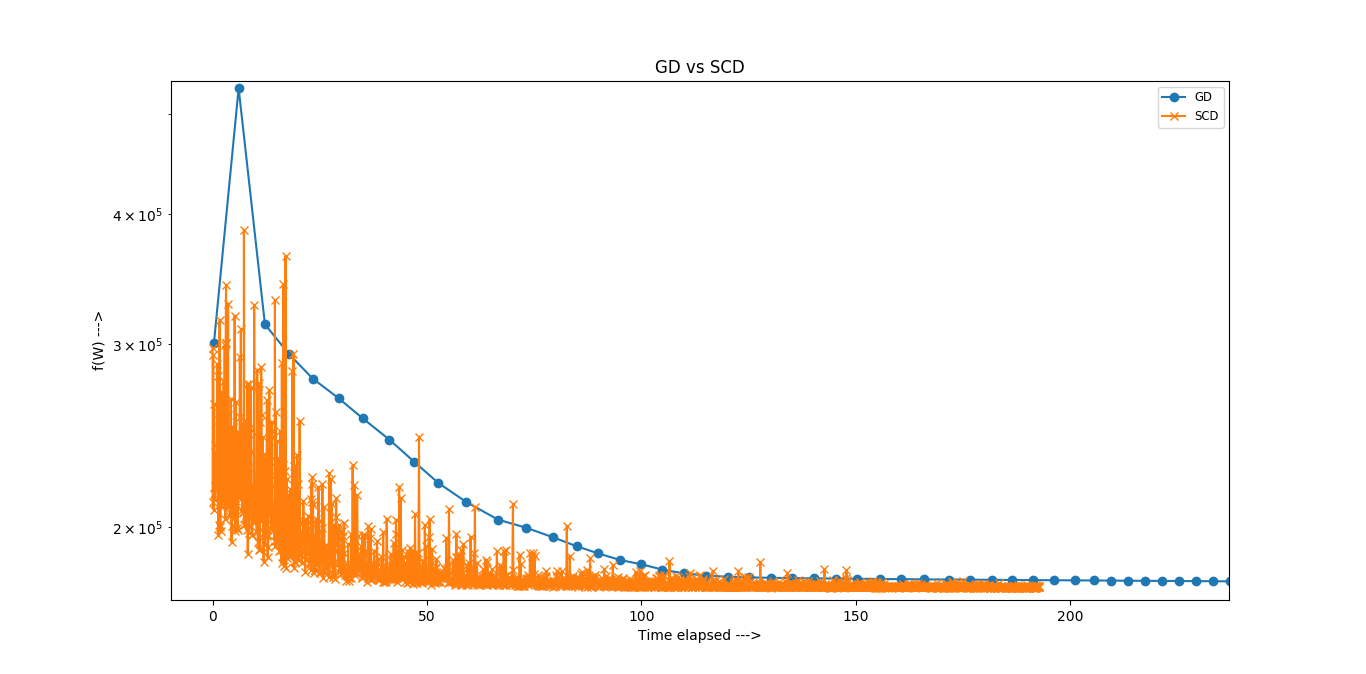
\includegraphics[width=1.2\columnwidth]{GdVsScdElapsed.png}%

\caption{GD And SCD with Time Elapsed on X and Objective f(W) on Y axis.}%
\label{fig:GD3}%
\end{figure}
\begin{figure}[th]%
\centering
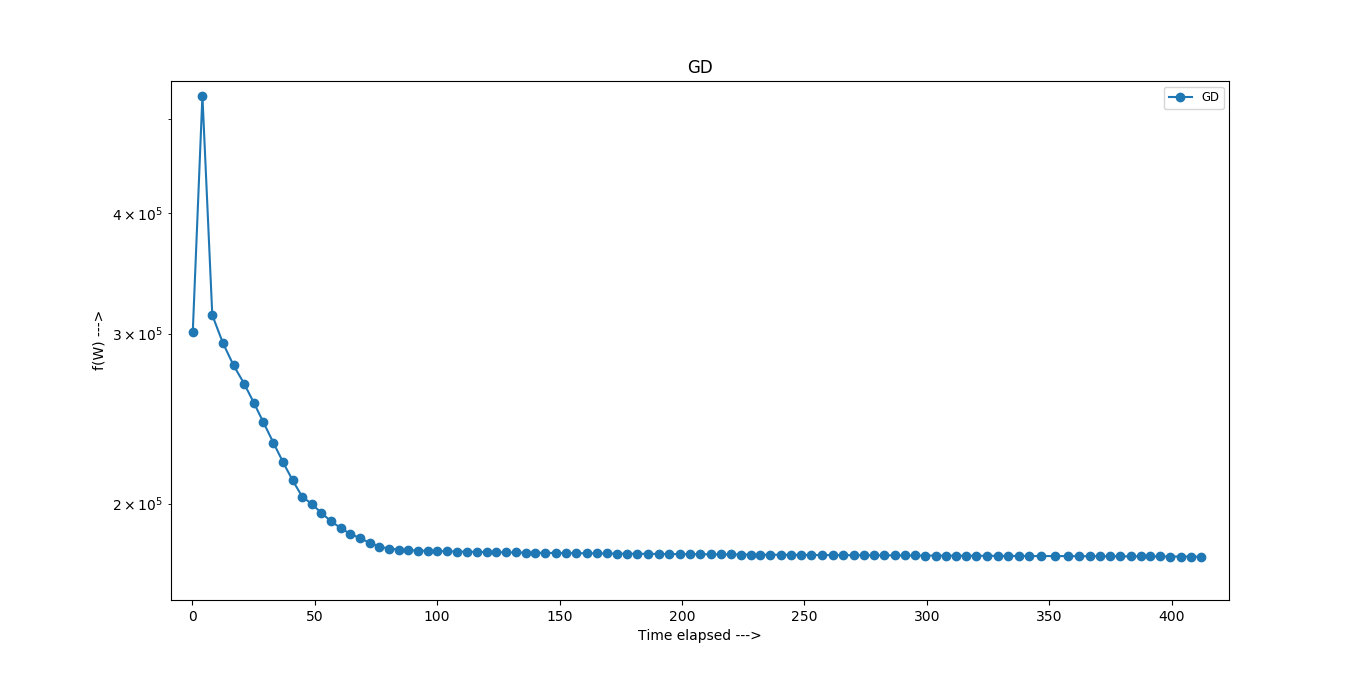
\includegraphics[width=1.2\columnwidth]{GD-elapsed.png}%

\caption{Gradient Descent with Time Elapsed on X and Objective f(W) on Y axis.}%
\label{fig:GD1}%
\end{figure}
\begin{figure}[th]%
\centering
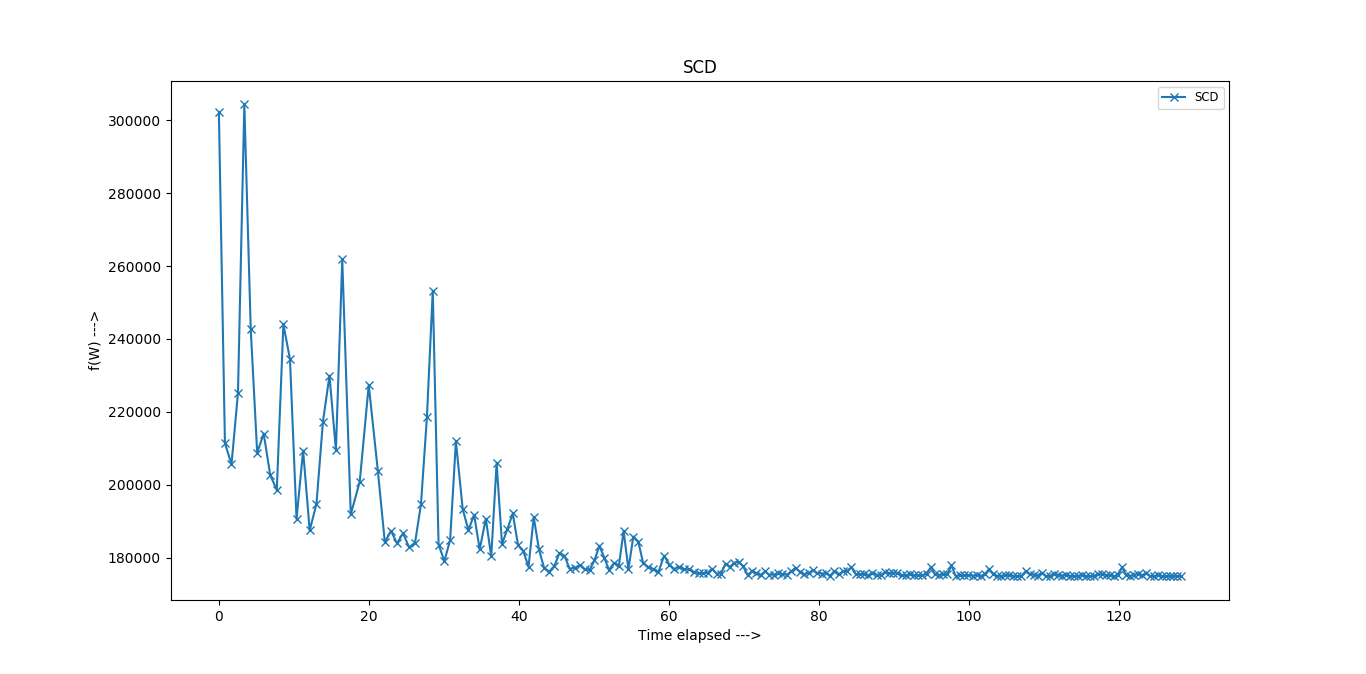
\includegraphics[width=1.2\columnwidth]{SCD-elapsed.png}%

\caption{SCD with Time Elapsed on X and Objective f(W) on Y axis.}%
\label{fig:SCD1}%
\end{figure}


\newpage
(Part VI)

The difference observed in graph with Theoretical Time Vs Time Elapsed is that the theoretical time taken by SCD is much much smaller than that taken by GD, As one iteration does n*d work in GD which is $300K * 54$ and takes d work in SCD which is $54$. This shows that SCD takes much less time to converge where as time elapsed doesn't involve the work done per iteration as shown in figure 5. So according to theoretical time also SCD reduces $f(W)$ faster than GD.

\begin{figure}[th]%
\centering
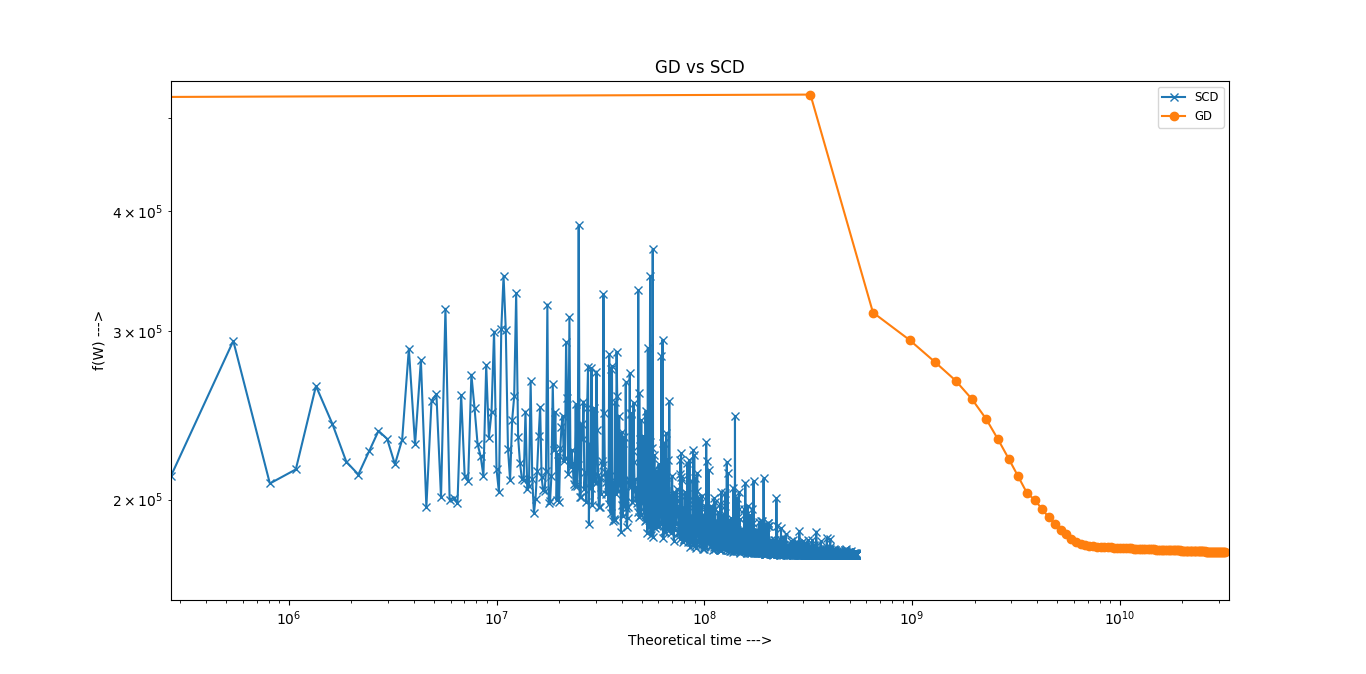
\includegraphics[width=1.1\columnwidth]{GdVsSCDTheo.png}%

\caption{GD And SCD with Theoretical Time Elapsed on X and Objective f(W) on Y axis.}%
\label{fig:GD4}%
\end{figure}

\begin{figure}[th]%
\centering
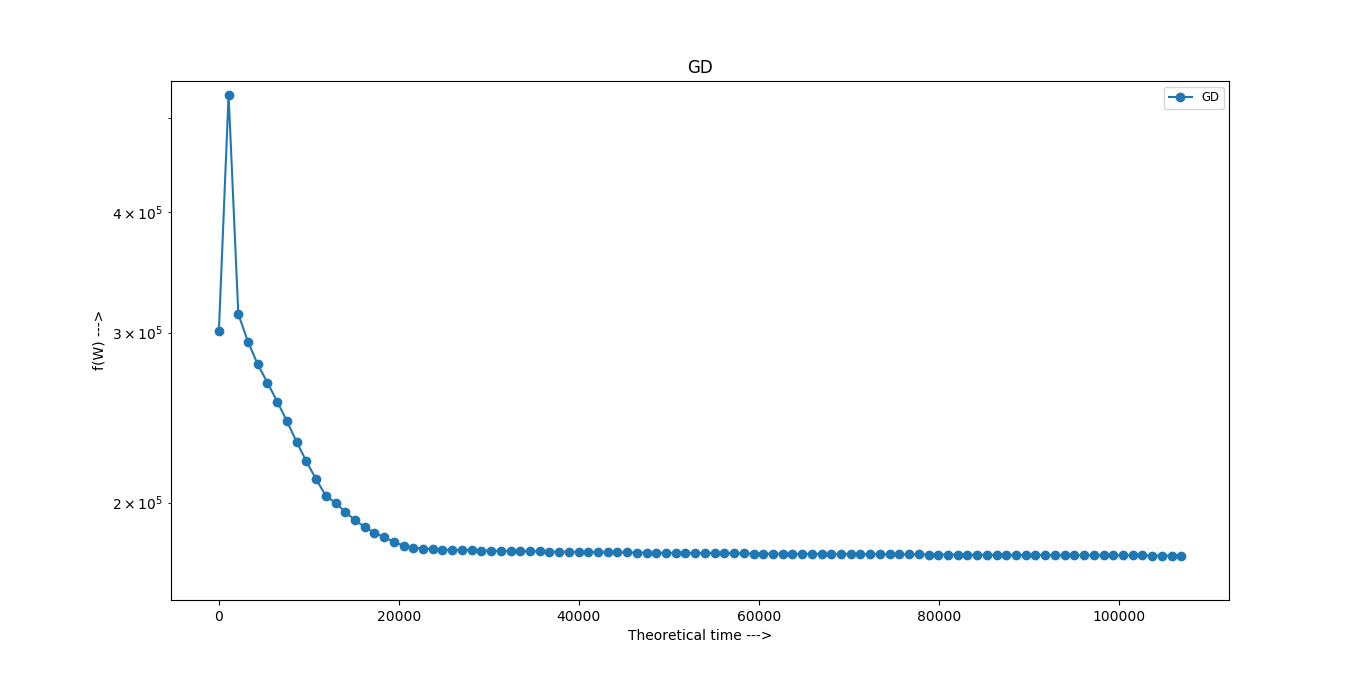
\includegraphics[width=1.2\columnwidth]{GD-theo.png}%

\caption{GD with Theoretical Time Elapsed on X and Objective f(W) on Y axis.}%
\label{fig:GD2}%
\end{figure}

\begin{figure}[th]%
\centering
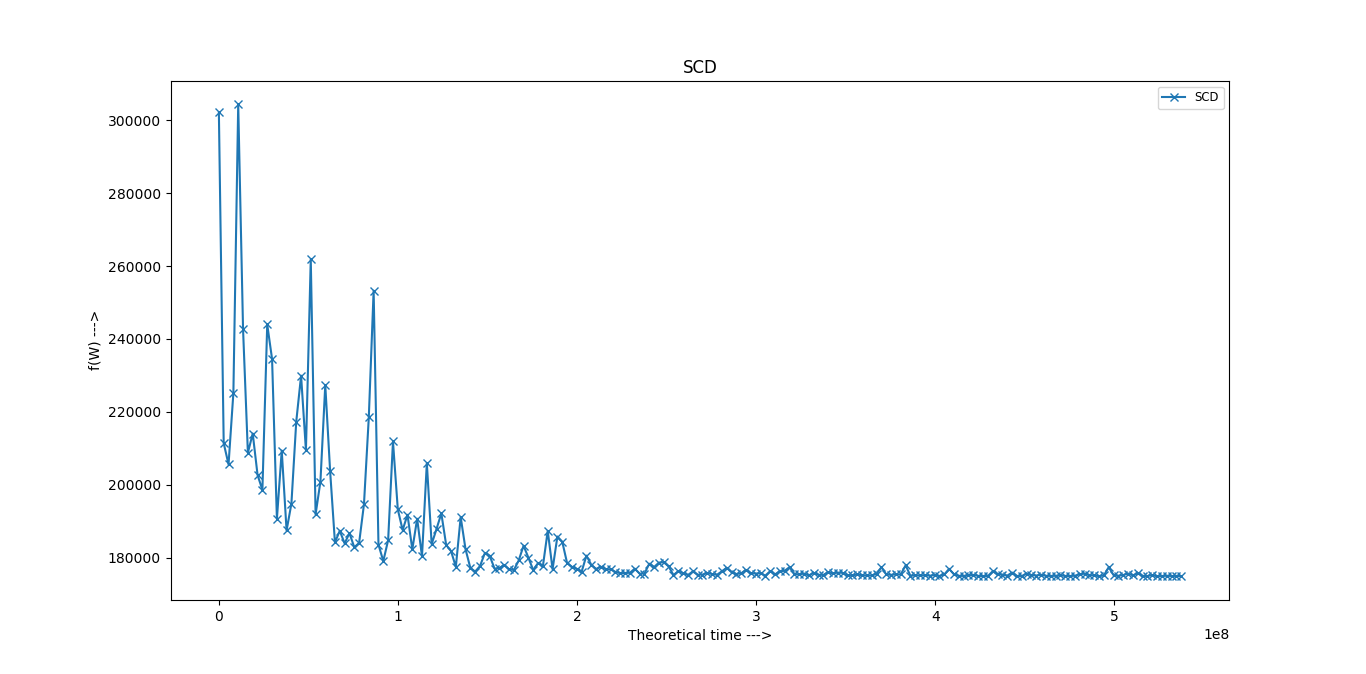
\includegraphics[width=1.2\columnwidth]{SCD-theo.png}%

\caption{SCD with Theoretical Time Elapsed on X and Objective f(W) on Y axis.}%
\label{fig:SCD2}%
\end{figure}

\end{mlsolution}
          
\end{document}